\documentclass[t]{beamer} % t is for TOP align (delete if we want to center the content on the slides)
% SEMB - misra c

\mode<presentation>
{
  \usetheme{Dresden}      % or try Darmstadt, Madrid, Warsaw, ...
  \usecolortheme{whale} % or try albatross, beaver, crane, ...
  \usefonttheme{serif}  % or try serif, structurebold, ...
  \setbeamertemplate{navigation symbols}{}
  \setbeamertemplate{caption}[numbered]
} 

\usepackage[most]{tcolorbox}
\usepackage{graphicx}
\usepackage{picture}

\usepackage[english]{babel}
\usepackage[utf8x]{inputenc}
\usepackage{multicol}
\usepackage{multirow}
\usepackage{tabularx}
\usepackage{listings}
\usepackage{color}
\definecolor{dkgreen}{rgb}{0,0.6,0}
\definecolor{gray}{rgb}{0.5,0.5,0.5}
\definecolor{mauve}{rgb}{0.58,0,0.82}
\lstset{frame=tb,
  language=C,
  aboveskip=3mm,
  belowskip=3mm,
  showstringspaces=false,
  columns=flexible,
  basicstyle={\small\ttfamily},
  numbers=none,
  numberstyle=\tiny\color{gray},
  keywordstyle=\color{blue},
  commentstyle=\color{dkgreen},
  stringstyle=\color{mauve},
  breaklines=true,
  breakatwhitespace=true,
  tabsize=3,    
}
\newtcolorbox{myquote}{colback=yellow!20!white,colframe=yellow!75!black,grow to right by=-10mm,grow to left by=-10mm,
    boxrule=0pt,boxsep=0pt,breakable} \makeatletter

\graphicspath{ {./} }

\title[SEMB/SETR]{MISRA-C}
\author{Alena Tesařová, Stylianos Tsagkarakis, Vasileios Konstantaras}
\institute{Faculty of Engineering of the University of Porto}
\date{\today}

%\AtBeginSection[]
%{
%  \begin{frame}<beamer>
%    \frametitle{Outline}
%    \tableofcontents[currentsection,currentsubsection]
%  \end{frame}
%}

% --------- NOTES MISRA ---------------
% This is the recommended link:
% 1. https://www.embedded.com/introduction-to-misra-c/

% Very good page:
% 2. https://www.perforce.com/resources/qac/misra-c-cpp
% 3. https://www.perforce.com/blog/qac/3-examples-better-embedded-coding-misra

% School(FEUP) presentation:
% 4. https://sigarra.up.pt/feup/pt/conteudos_service.conteudos_cont?pct_id=663730&pv_cod=03Lam5MauaVa
% -------- END NOTES ------------

% 2 SLIDES
% Outline
% 1. Introduction + Motivation
%       1. What is MISRA-C
%       2. Who created it
%       3. Why it was created (general)
%       4. Examples of malfunction of embedded systems
%
% 2 SLIDES
% 2. Guideline Classification
%       Guideline Types
%       Rule Analysis
%       Guideline Categories
%           Mandatory
%           Required
%           Advisory
%           Dis-applied
% RULES
% 1 - Environment
% 2 – Language Extensions
% 3 – Documentation
% 5 – Identifiers
% 6 - Types
% 7 – Constants
% 8 – Declarations & Definitions
% 9 – Initialization
% 10 – Arithmetic Type Conversions
% 12 – Expressions
% 13 – Control Statements
% 14 – Control Flow
% 16 – Functions
% 17 – Pointers & Arrays
% 18 – Structures & Unions
% 20 – Standard Libraries
%
%
% Compliance checking
%       - compilers etc.
%       - Helix
%       - Automotive, ..
% Conclusion


\begin{document}


\begin{frame}
    \titlepage
\end{frame}

\begin{frame}{Outline}
    \tableofcontents
\end{frame}

\section{Introduction}

\begin{frame}{What is MISRA-C?}
    %\begin{block}{}
  		     MISRA-C is a set of software development guidelines for the programming language C in critical systems, developed by \textbf{M}otor \textbf{I}ndustry \textbf{S}oftware \textbf{R}eliability \textbf{A}ssociation.
  		        \begin{itemize}
  		            \item 1st Edition 1998 (127 coding rules)
  		            \item 2nd Edition 2004 (142 coding rules)
  		            \item 3rd Edition 2012 (143 coding rules)
  		            \item 2016 \& 2020 Amendment
  		        \end{itemize}
  		        %  C is widely used in Embedded Systems because of the easy access to hardware, efficient run-time performance and low memory requirements but on the contrary C:
  		        %\end{block}  
  		        \begin{block}{ Use of C in Embedded Systems}
     		        \begin{columns}
  		            \column{0.5\textwidth}
     		            \begin{itemize}
                            \begin{footnotesize}
          		                \item[$+$] easy access to hardware
          		                \item[$+$] efficient run-time performance
          		                \item[$+$] low memory requirements
                        \end{footnotesize}
                    \end{itemize}
		            \column{0.5\textwidth}
                        \begin{footnotesize}
         		            \begin{itemize}
          		                \item[$-$] has limited run-time checking
          		                \item[$-$] a programmer can easily make a mistake
          		                \item[$-$] compilers might contain errors
          		            \end{itemize}
                        \end{footnotesize}
                    \end{columns}
                    \end{block}  
  	  
\end{frame}
% later
\begin{frame}
    \begin{block}{}
  		    Today, MISRA is used in fields such as:  
  		        \begin{itemize}
  		            \item Automotive Industry
  		            \item Railway Systems
  		            \item Aerospace Industry
  		            \item Telecommunications
  		            \item Medical Devices
  		        \end{itemize}
  	  \end{block}
  		     Using MISRA standards companies ensure their code is:
  		        \begin{itemize}
  		            \item Safe
  		            \item Secure
  		            \item Reliable
  		            \item Portable
  		        \end{itemize}{}
 	
\end{frame}

\section{Guideline Classification}
% NOTES
% Now, let s get to classification of the guideline. First of all it's necessary to mention that guideline is described as either a rule or a directive. There is a main difference between these 2 classifications and that is a definition of the requirements. 

%Directives are not often well defined or refers to requirements on process or documentation. However the majority of guidelines are classified as rules. Regarding rules -- compliance is depended entirely on the source code and not on any design feature or documentation.

%Interesting is that earlier version of the MISTRA Guidelines used no such distinction, and, in fact, consist almost entirely of rules. 

%On the slide there are two examples. The first example is a directive and says that we should document the implementation on which the output depends. The second one is about functions atof, atoi and atoll that we should avoid using because these functions have undefined behaviour associated with them when the string cannot be converted.

\begin{frame}{Guideline types}
%	\begin{itemize}
% \begin{block}{}
	    %\begin{itemize}
	     %  \item[$-$] 
	        $-$ Directives
	            \begin{itemize}
	                \item does not have to be well defined
	                \item often address \textit{process} or \textit{documentation} requirements
	            \end{itemize}{}
	            \begin{figure}[h]
                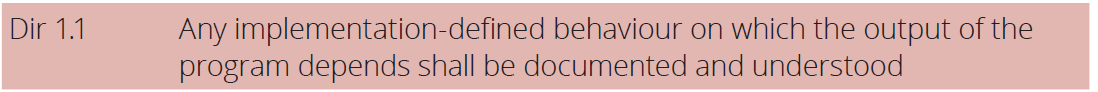
\includegraphics[width=\textwidth]{dirdoc.PNG}
                \end{figure}
	         $-$ Rules
	            \begin{itemize}
	                \item formally and well defined
	                \item compliance is depended entirely on the source code %and not on any design feature or documentation
	            \end{itemize}
	             \begin{figure}[h]
                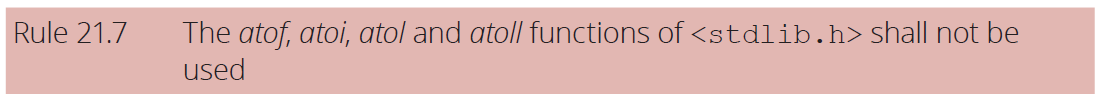
\includegraphics[width=\textwidth]{rule1.PNG}
                \end{figure}
	        %\item[$-$] Dis-applied - didn't find
	   % \end{itemize}{}
%	\end{itemize}
%\end{block}
\end{frame}

% NOTES starts: 1:35
% Every rule is described as either mandatory, required or advisory depending whether a guideline may be violated or not and whether a deviation is required. In the picture below we can see an example of how the categorization looks in the guideline. 

%Mandatory are guidelines for which violation is never permitted. Regarding required guidelines  -- these can only be violated when are supported by a deviation which must follow set of clear restrictions. Last category is advisory -- these are recommendations that should be followed as far as is reasonably practical. 

%Some categories can be treated as different categories depending on the project. For example some advisory guidelines can be ignored altogether or on the other hand they can be treated as Mandatory or Required. In version from 2016 we can find a table with permissions telling us which categories are allowed to be treated as different categories. 

\begin{frame}{Guideline Classification}
%	\begin{itemize}
 \begin{block}{ Guideline categories}

	    \begin{itemize}
	        \item[$-$] Mandatory
	            \begin{itemize}
	                \item deviations and violation are not permitted
	            \end{itemize}{}
	        \item[$-$] Required
	            \begin{itemize}
	                \item mandatory requirements
	                \item can be treated as Mandatory
	                \item deviation allowed, but must follow some formalization
	            \end{itemize}{}
	        \item[$-$] Advisory
	            \begin{itemize}
	                \item recommendations, can be treated as Mandatory or Required
	            \end{itemize}{}
	        %\item[$-$] Dis-applied - didn't find
	    \end{itemize}{}
	     \begin{figure}[h]
                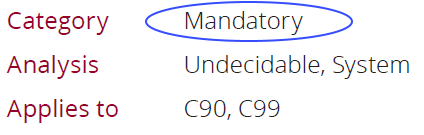
\includegraphics[width=0.5\textwidth]{example.PNG}
                \end{figure}
%	\end{itemize}
\end{block}
\end{frame}
% NOTES starts 2:54
% The last classification that was already seen in the previous picture is the decidability of the rules. We can often ask "Does this code comply with this rule?". Unfortunately there are some rules for which an answer can not be provided in all circumstances and that is the reason of this classification.

%A rule is decidable if it is always possible to answer the question with Yes or No so it's always possible to verify the compliance. Although undecidable rules are the rules where we can not guarantee the response with yes or no. 

% Examples
%First example talks about distinction of identifiers in the same scope -- this we can always verify that by the compiler so it is a decidable rule. On the other hand, next example talks about unreachable code that the project shall not contain. It is an undecidable rule because all compilers can not prove that.

\begin{frame}{Guideline Classification}
 \begin{block}{Decidability of rules}
	 \begin{itemize}
	     \item Decidable -- can be verified by a program
	     \item Undecidable -- if it is not decidable
	     % A rule is decidable if it is possible for a program to answer the question with a “yes” or a “no” in every case and undecidable otherwise
	 \end{itemize}
\end{block}	 
\begin{block}{Example of a decidable rule}
\textbf{Rule 5.2}: identifiers declared in the same scope and namespace shall be
distinct 
\end{block}

\begin{block}{Example of a undecidable rule}
\textbf{Rule 2.1}: A project shall not contain unreachable code
\end{block}

\end{frame}


\begin{frame}{Organization of the rules}
% NOTES starts 3:55
% MISRA contains rules which are classified into 21 categories. We will not go throw all of them. We picked just some to present to you that we liked the most.

\begin{columns}
\column{0.5\textwidth}
\begin{itemize}
\begin{footnotesize}
\item 1. Environment
\item 2. Language Extensions
\item 3. Character set
\item 4. Documentation
\item 5. Identifiers
\item 6. Types
\item 7. Constants
\item 8. Declarations \& Definitions
\item 9. Initialization
\item 10. Arithmetic Type Conversions
\end{footnotesize}
\end{itemize}

\column{0.5\textwidth}
\begin{itemize}
\begin{footnotesize}
\item 11. Pointer Type Conversions
\item 12. Expressions
\item 13. Control Statements
\item 14. Control Flow
\item 15. Switch statements
\item 16. Functions
\item 17. Pointers \& Arrays
\item 18. Structures \& Unions
\item 19. Preprocessing directives
\item 20. Standard Libraries
\item 21. Run-time failures
\end{footnotesize}
\end{itemize}

\end{columns}

\end{frame}
\section{MISRA-C rules}


% NOTES starts 4:05 - 4:34
% I picked the rule in comments section. It says Line-splicing shall not be used in double slash comments. The usage can also be seen in the code example. If we put a character backslash on the end of comment than the new line becomes a part of the comment and this can result to a loss of some important code and problems in the future. This rules is classified as required.

\begin{frame}[fragile]{8.3 Comments}
\begin{block}{\textbf{Rule 3.2:} Line-splicing shall not be used in // comments}


\begin{lstlisting}
extern bool_t b;
void f ( void )
{
    uint16_t x = 0; // comment \
    if ( b )
    {
        ++x;  /* This is always executed */
    }
}
\end{lstlisting}
\begin{itemize}
    \item required
    \item the new line becomes a part of the comment
\end{itemize}{}

\end{block}{}
\end{frame}
\begin{frame}[fragile]{8.5 Identifiers}
\begin{block}{\textbf{Rule 5.3:} A typedef name shall be a unique identifier.}
The following example is NOT acceptable:
    \begin{lstlisting}
        { typedef unsigned char uint8_t;}
        { typedef unsigned char uint8_t;} //NOT compliant - redefinition
        { unsigned char uint8_t;} //NOT compliant - reuse of int8_t
    \end{lstlisting}
    \begin{itemize}
        \item required
        \item redefinition of typedef is not allowed
    \end{itemize}
\end{block}{}

\end{frame}

% ### Rule 13.3

% A function call is considered to be a side effect for the purposes of this rule
% - The increment or decrement operator is a function call by itself.

% - It can significantly impair the readability of the code
% - It is clearer to use these operations in isolation from any other operators

\begin{frame}[fragile]{8.13 Side Effects}
\begin{block}{\textbf{Rule 13.3:} A full expression containing an increment(++) or decrement(--) operator should have no other potential side effects other than that caused by the increment or decrement operator}
    \begin{lstlisting}
        u8a = ++u8b + u8c--;
        // is clearer when written as the following sequence:
        ++u8b;
        u8a = u8b + u8c;
        u8c--;
    \end{lstlisting}
     \begin{itemize}
        \item advisory
    %    \item clearly arranged
    \end{itemize}
\end{block}{}
\begin{block}
 
\end{block}{}

\end{frame}

% ### Rule 15.1
% This can lead programs that are unstructured and extremely difficult to understand. So it is not only hard to maintain them but also can lead to uncontrolled programs that we cannot predict the control flow.

% ### Rule 15.2
% This specific rule helps to maintain the "natural" flow of the program and it also helps to minimize visual code complexity.

% ### Conclusion between rules
% Here we can see the difference between a Required rule and an Advisory rule. Although we are suggested not to use goto, we can use it only if we comply with some regulations that ensure further safety to our program.

\begin{frame}[fragile]{8.15 Control Flow}
\begin{block}{\textbf{Rule 15.1:} Advisory: The goto statement \textbf{should not} be used.}
\end{block}{}
\begin{block}{\textbf{Rule 15.2:} Required: The goto statement \textbf{shall} jump to a label declared later in the same function.}
\end{block}{}

     \begin{lstlisting}
        L1: ++i;
            if i>10
                goto L2; // compliant
        L2: ++j;
            if j>20
                goto L1; // NOT-compliant
    \end{lstlisting}
 
\end{frame}

% ### Compliance checking

% 1. You need to know the MISRA coding rules pertinent to which version of C or C++ you’re using.
% 2. Continuously inspecting your code for violations is the best way to improve quality.
% 3. Embedded systems come with legacy codebases. By setting baselines, you can focus on making sure your new code is compliant.
% 4. You could have hundreds or even thousands of violations in your code. That’s why it’s important to prioritize rule violations based on risk severity. Some static code analysis tools can do this for you.
% 5. Sometimes there are exceptions to the rule. But when it comes to compliance, every rule deviation needs to be well-documented.
% 6. Keep an eye on how MISRA compliant your code is. Using a static code analyzer makes this easier by automatically generating a compliance report.
% 7. Choosing the right static code analyzer makes everything else easy. It takes care of scanning your code — new and legacy — for violations. It prioritizes vulnerabilities based on risk.

\section{Compliance checking}
\begin{frame}[fragile]{Using MISRA-C (1) }
    \begin{block}{Things to take into consideration to comply with MISRA.}     
    \begin{enumerate}
            \item Know the Rules
            \item Check Your Code Constantly
            \item Set Baselines
            \item Prioritize Violations Based on Risk
            \item Document Your Deviations
            \item Monitor Your MISRA Compliance
            \item Choose the Right Static Code Analyzer
         \end{enumerate}
    \end{block}  
\end{frame}

% ### Compilers
% The compiler’s optimization options should be reviewed and selected carefully in order to ensure that an appropriate balance between execution speed and code size has been obtained

\begin{frame}[fragile]{Using MISRA-C (2) }
    \begin{block}{Compliance Matrix} 
    \begin{enumerate}
        \begin{footnotesize}
            \item Cross - compiler
            \item Different Tools
            \item Manual Inspection
        \end{footnotesize}
    \end{enumerate}
    \begin{footnotesize}If any specific restrictions are omitted there should be full justification.\end{footnotesize}
    \begin{figure}
        \centering
        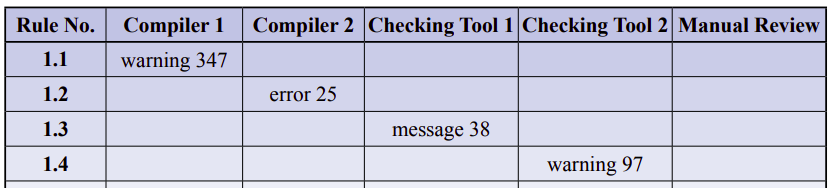
\includegraphics[scale=0.36]{compliance_matrix.png}
        \caption{Compliance Matrix}
        \label{fig:my_label}
    \end{figure}
    \end{block}  
\end{frame}

% ### Helix
% Helix QAC is a commercial static code analysis software tool. You can see here, you have the code on the top left, and the report on the bottom, referencing every rule.

\begin{frame}{Helix static analysis tool}
    \begin{figure}
        \centering
        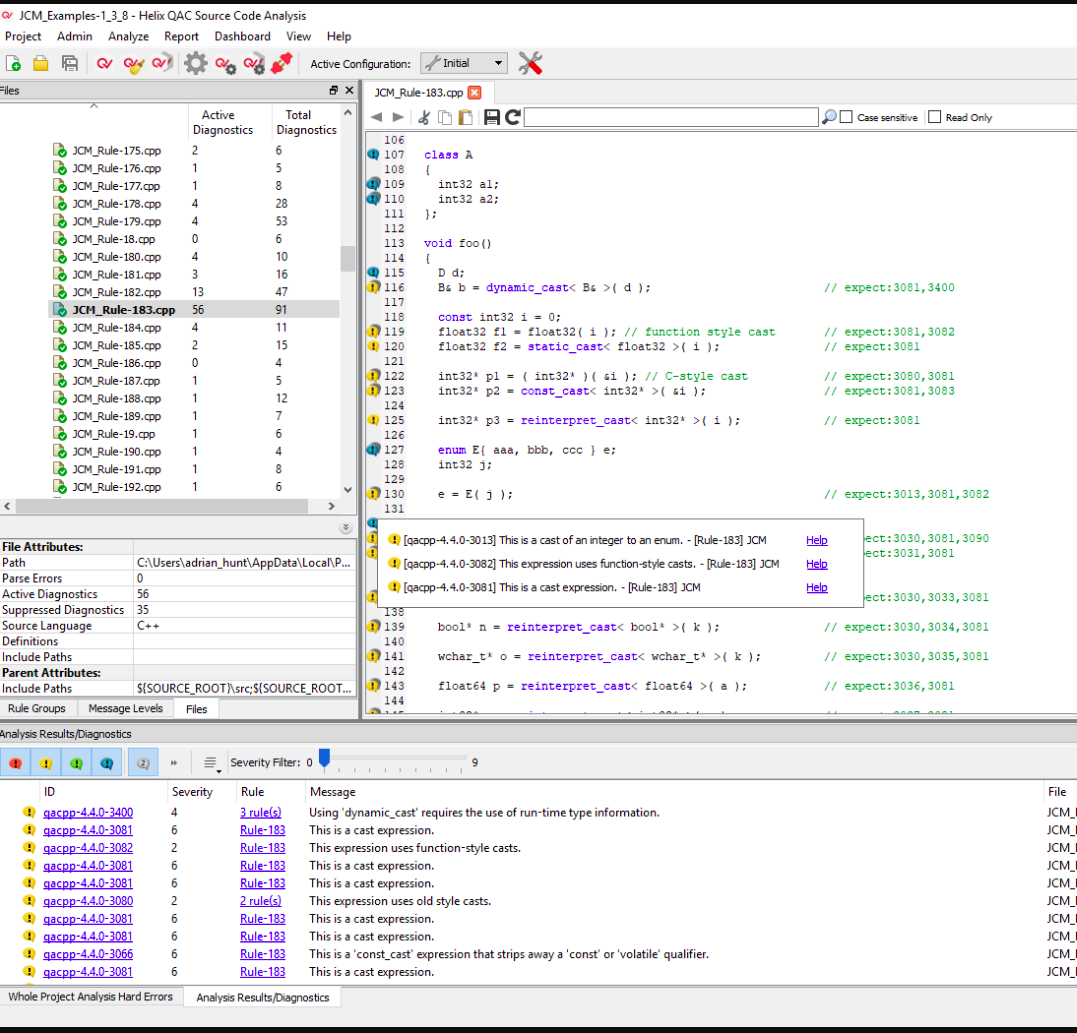
\includegraphics[scale=0.22]{helix_IDE.png}
       % \caption{Helix IDE}
        \label{fig:my_label}
    \end{figure}
\end{frame}


\section{Conclusion}
\begin{frame}{Conclusion}

\begin{block}{Why MISRA C?}
\vspace{10pt}
\begin{itemize}
    \item Maximizes effectiveness
    \item Documenting the disadvantages and limitations
    \item Guiding developers to use them in their advantage
\end{itemize}
\vspace{12pt}
\begin{center}

’’ Using C weaknesses to your own gain. ’’

\end{center}
%MISRA tries to maximize the effectiveness of C by documenting the disadvantages and limitations of the language and guiding the developers on how to use them in their advantage. This way it uses it's weaknesses to it's own gain.%

\end{block}{}

\end{frame}

\begin{frame}
\begin{block}{References}
\begin{thebibliography}{Per00}
\small{
	\bibitem[1]{misra}
	\emph{MISRA C:2012 - Addendum 2:  Coverage of MISRA C:2012 against ISO/IEC TS 17961:2013 "C Secure", ISBN 978-906400-18-7 (PDF), Second Edition, January 2018.}
	
	\bibitem[1]{misra}
	\emph{MISRA C:2004 Permits:  Deviation permits for MISRA compliance, ISBN 978-906400-14-9 (PDF), Edition 1, April 2016.}
	
	\bibitem[2]{misra2}
    \emph{Introduction to MISRA C. [Online, last update 1.7.2002]. URL \url{https://www.embedded.com/introduction-to-misra-c/}}
    
    \bibitem[3]{misra3}
    \emph{3 Examples of Better Embedded Coding with MISRA [Online, last update 6.1.2020] \url{https://www.perforce.com/blog/qac/3-examples-better-embedded-coding-misra}}
    
    \bibitem[4]{misra4}
    \emph{MISRA C and MISRA C++
    \url{https://www.perforce.com/resources/qac/misra-c-cpp}}
}
\end{thebibliography}
\end{block}{}
\end{frame}

\begin{frame}
%\begin{block}
\vspace{\fill}
    \begin{center}
        \large{
            % \textbf{
                ’’ MISRA-C will make your code not MISRAble ’’
            % }
        }
    \end{center}
%\end{block}
\end{frame}

\end{document}

